\section{System Design}
\label{sec:system}

\subsection{Overall Architecture}
\label{sec:overall-architecture}

ZhuLong is built on Cline-CLI \cite{cline2024cline}, an open-source framework for autonomous coding agents, extended with EDA-specific retrieval, documentation, and execution capabilities. Throughout, we call the resulting runtime an \textbf{ICL-type autonomous agent}: an agent that decides its own next action, keeps no explicit posterior, and maintains its belief state implicitly by in-context learning, as formalized in Section~\ref{sec:grounding-theory}. We choose Cline-CLI for its mature permission controls, human-in-the-loop support, and enterprise readiness. As shown in Figure~\ref{fig:architecture}, the system comprises three components: the LLM-based agent runtime, the API knowledge base, and the EDA execution environment. The agent interacts with these components through three MCP tools, while an offline \textbf{API self-exploration mechanism} pre-augments the API knowledge base before runtime.
% ZhuLong基于Cline-CLI \cite{cline2024cline}构建，这是一个开源自主代码智能体框架，我们扩展了EDA特定的检索、文档查阅和执行能力。选择Cline-CLI是因为其成熟的权限控制、人在闭环支持和企业级就绪能力。如图~\ref{fig:architecture}所示，系统包括三个组件：基于LLM的智能体运行时、API知识库和EDA执行环境。智能体通过三个MCP工具与这些组件交互，离线\textbf{API自探索机制}在运行前预增强API知识库。

\begin{figure*}[t]
\centering
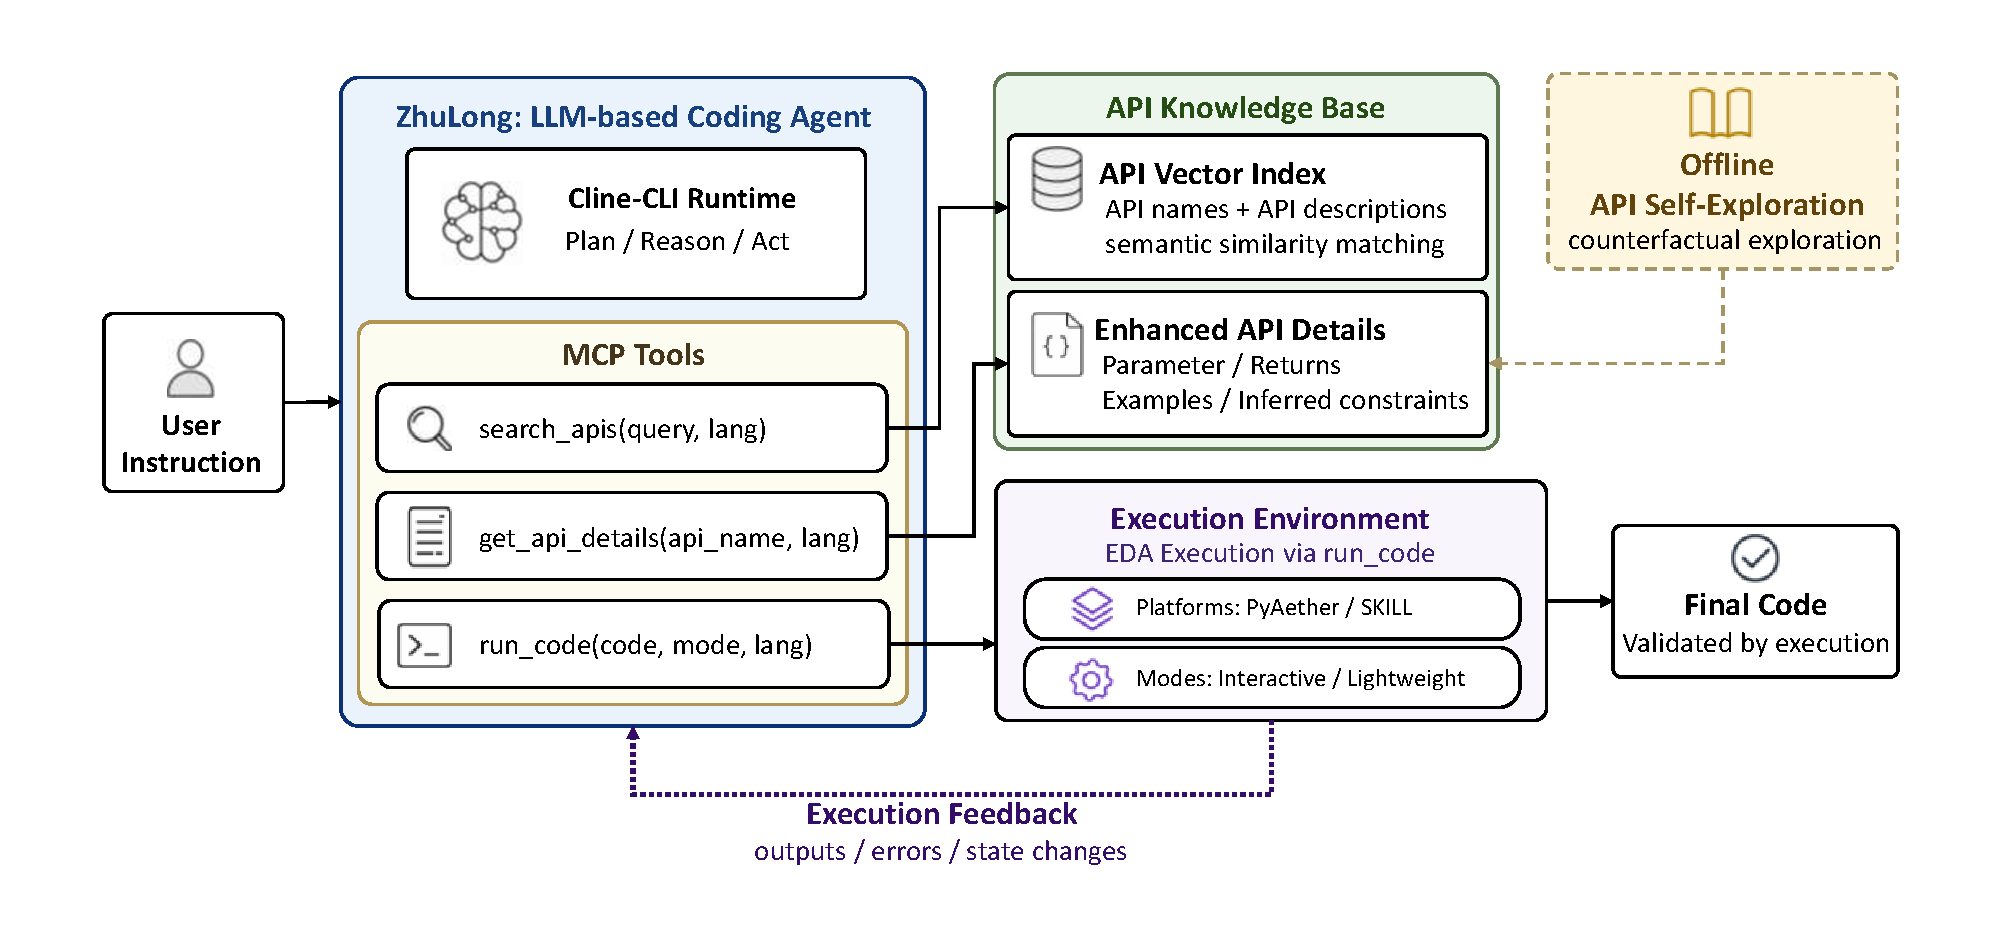
\includegraphics[width=0.9\textwidth]{figures/zhulong_arch_2.pdf}
\caption{ZhuLong system architecture. The agent interacts with API retrieval, enhanced documentation, and EDA execution via three unified MCP tools. Offline self-exploration augments the knowledge base before runtime, and execution feedback supports iterative refinement.}
% ZhuLong系统架构。智能体通过三个统一的MCP工具与API检索、增强文档和EDA执行环境交互。离线自探索在运行前增强知识库，执行反馈支持迭代优化。
\Description{Block diagram of ZhuLong's three components: the LLM agent runtime, the API knowledge base (search and retrieval), and the EDA execution sandbox. The runtime calls three MCP tools -- search_apis, get_api_details, and run_code -- with execution feedback looped back for iterative refinement; an offline self-exploration step pre-augments the knowledge base.}
\label{fig:architecture}
\end{figure*}

\subsection{Three MCP Tools}
\label{sec:mcp-tools}

ZhuLong extends three MCP tools \cite{mcp2024protocol}, each accepting a unified \texttt{lang} parameter (\texttt{pyaether}, \texttt{skill}, or \texttt{tcl}) to support all three platforms with identical agent logic:
% ZhuLong扩展了三个MCP工具 \cite{mcp2024protocol}，每个工具接受统一的\texttt{lang}参数（\texttt{pyaether}或\texttt{skill}），以相同智能体逻辑支持两个平台：

\begin{itemize}
    \item \texttt{search\_apis(query, lang)} retrieves relevant APIs via semantic and keyword-based search. We index APIs by name and description using BGE-M3 embeddings \cite{bge2024} with FAISS \cite{douze2024faiss} for efficient similarity search, returning the top-$K$ results ($K=5$ by default) with confidence scores and descriptions.
    % \texttt{search\_apis(query, lang)}通过语义和关键词检索相关API。我们使用BGE-M3嵌入 \cite{bge2024}对API名称和描述建索引，FAISS \cite{faiss2017}支持高效相似度搜索，返回top-$K$结果（默认$K=5$），附带置信度分数和描述。
    
    \item \texttt{get\_api\_details(api\_name, lang)} fetches comprehensive documentation for a specified API, including parameter types, return values, and examples. The returned documentation is augmented by the offline API self-exploration mechanism (Section~\ref{sec:selfdoc}) when available, enriching incomplete specifications with constraints and usage patterns discovered via sandbox exploration.
    % \texttt{get\_api\_details(api\_name, lang)}获取指定API的完整文档，包括参数类型、返回值和示例。当可用时，返回的文档由离线API自探索机制（第~\ref{sec:selfdoc}节）增强，补充通过沙盒探索发现的约束和使用模式。
    
    \item \texttt{run\_code(code, mode, lang)} executes the generated code in the EDA environment. It supports two modes: (1) \textbf{lightweight}—runs in a sandboxed environment without a GUI session (standalone PythonE for PyAether, or SKILL in batch mode for Virtuoso), capturing outputs, errors, and state changes for iterative refinement; (2) \textbf{interactive}—runs inside an open EDA session via the agent-EDA bridge (socket communication), enabling operations on unsaved layouts and schematics.
    % \texttt{run\_code(code, mode, lang)}在EDA环境中执行生成的代码。支持两种模式：（1）\textbf{轻量模式}——在沙盒化环境中运行，无需GUI会话（PyAether使用独立PythonE环境，Virtuoso使用SKILL批处理模式），捕获输出、错误和状态变化供迭代优化使用；（2）\textbf{交互模式}——通过agent-EDA桥接（socket通信）在已打开的EDA会话内运行，支持操作未保存的版图和原理图。
\end{itemize}

\subsection{Agent Workflow}
\label{sec:agent-workflow}

The agent iteratively refines its output through execution feedback \cite{cline2024cline}. A typical trajectory begins with reasoning over the user instruction, followed by API retrieval via \texttt{search\_apis} when needed. Candidate APIs are then inspected via \texttt{get\_api\_details}, and code is generated accordingly. The agent executes the code via \texttt{run\_code}, observes the result, and re-plans—revising the code, retrieving alternative APIs, or terminating. This loop continues until success or the agent determines further attempts are unlikely to succeed. The agent is not constrained to a fixed sequence; it may skip retrieval when it already knows the required API, or conduct multiple rounds of retrieval when initial results lack confidence.
% 智能体通过执行反馈迭代优化其输出 \cite{cline2024cline}。典型轨迹始于对用户指令的推理，需要时通过\texttt{search\_apis}检索API，然后通过\texttt{get\_api\_details}查阅候选API的文档，据此生成代码。智能体通过\texttt{run\_code}执行代码、观察结果并重规划——修改代码、检索替代API或终止。此循环持续至成功或智能体判断继续尝试不太可能成功。智能体不受固定序列约束——已知所需API时可跳过检索，初始结果置信度不足时可进行多轮检索。

\subsection{Offline API Self-Exploration (Complementary)}
\label{sec:selfdoc}

EDA API documentation is often incomplete, omitting parameter constraints, return structures, and error conditions. Prior work addresses these gaps through retrieval-based augmentation \cite{pu2024rag} or static knowledge graphs \cite{liu2025layoutcopilot}---both of which rely on what is already documented. As the theoretical framing of Section~\ref{sec:grounding-theory} makes precise, such mechanisms enrich only the L1--L3 facts the observation channel can return; they are therefore complementary to---and bounded by---the observation of L4 that requires acting on the live design. We accordingly position self-exploration as an efficiency and robustness mechanism, not as the primary accuracy driver.
% EDA工具的API文档往往不完整，省略参数约束、返回结构和错误条件。已有工作通过检索增强或静态知识图谱弥补文档缺口，但两者都依赖已有文档。
% 正如第~\ref{sec:grounding-theory}节的理论框架所指出的，这类机制只能丰富观测通道可返回的L1–L3事实；
% 因此它们相对"通过作用于实时设计来观测L4"是互补且有界的。我们将自探索定位为效率与鲁棒性机制，而非精度主驱动。

ZhuLong instead \textbf{proactively discovers} API behaviors through offline counterfactual experimentation in the sandbox. For each target API, the exploration agent reads available documentation, identifies gaps---e.g., unspecified parameter ranges, undocumented return fields, or ambiguous error semantics---and generates targeted test scripts to probe them. It executes these scripts via \texttt{run\_code}, observes outcomes, and iteratively refines a behavioral model of the API capturing parameter constraints, return structures, error conditions, and side effects. The exploration agent autonomously decides what to test next and when to stop, based on its current confidence. This offline process runs once per API; the enriched documentation is stored in the knowledge base and served at runtime via \texttt{get\_api\_details}, incurring no runtime overhead.
% ZhuLong转而通过沙盒中的离线反事实实验主动发现API行为。对每个目标API，探索智能体阅读现有文档、识别缺口、生成针对性测试脚本，通过run_code执行并观察结果，迭代细化API行为模型。探索智能体自主决定测试内容与停止时机。该离线过程每个API运行一次，增强文档存入知识库，运行时通过get_api_details提供，无额外开销。

\textbf{Implementation and cost.} The exploration agent targets the union of (i) APIs referenced by EDA-Eval-PyAether tasks and (ii) APIs whose official documentation omits at least one of parameter ranges, return types and structures, or error conditions. Each API is assigned a confidence score that accumulates the information gain of each probe; exploration terminates when the score exceeds threshold $\tau$, when two consecutive rounds contribute no new discriminated constraint, or when a per-API execution budget $M$ is exhausted. Generated test scripts are gated by EDA domain experts before execution to filter destructive operations, and discovered constraints are sanity-checked against vendor documentation where available. Exploration is a one-time offline cost per API (Table~\ref{tab:selfdoc-cost}).
% 实现与成本。探索以评测任务引用的API和官方文档缺失关键信息的API的并集为目标。每个API维护置信度分数，按每次探测的信息增益累积；当分数超过阈值、连续两轮无新增可判别约束、或单API执行预算耗尽时停止。生成的测试脚本在执行前经专家把关过滤破坏性操作。探索为每个API一次性的离线成本。

\begin{table}[htbp]
\centering
\caption{Self-exploration scale and cost (one-time, offline)}
\label{tab:selfdoc-cost}
\begin{tabular}{lc}
\toprule
\textbf{Item} & \textbf{Value} \\
\midrule
APIs targeted & [TBD] \\
APIs with $\geq 1$ discovered constraint & [TBD] \\
Average experiments per API & [TBD] \\
Average wall-clock per API (s) & [TBD] \\
Total offline wall-clock (h) & [TBD] \\
Human-reviewed test scripts & [TBD] \\
\bottomrule
\end{tabular}
\end{table}
% 表：自探索规模与成本（一次性、离线）。